
%(BEGIN_QUESTION)
% Copyright 2011, Tony R. Kuphaldt, released under the Creative Commons Attribution License (v 1.0)
% This means you may do almost anything with this work of mine, so long as you give me proper credit

An Allen-Bradley SLC 500 controls the start-up and shut-down of a large air blower (fan) with a pressurized lubrication oil sub-system to keep the blower bearings lubricated as they turn:

$$\includegraphics[width=15.5cm]{i04592x01.eps}$$

Analyze this control program, and then explain what each instruction does (including the practical function of each timer instruction).  Also, identify all conditions that will shut down this system (stopping the blower motor and the oil pump).

\vskip 20pt \vbox{\hrule \hbox{\strut \vrule{} {\bf Suggestions for Socratic discussion} \vrule} \hrule}

\begin{itemize}
\item{} Why is the oil pressure switch contact ({\tt I:1/4}) in-line with the {\tt LATCH\_RUN} seal-in contact rather than being in-line with the other shut-down permissive contacts (oil level pump vibration, etc.)?
\item{} Based on the color highlighting shown (red), what state is the program in?
\item{} Identify all the ``normal'' electrical switch contact statuses for each shutdown switch (e.g. vibration, temperature, etc.) based on an examination of the contact instructions in this program.
\end{itemize}

\underbar{file i04592}
%(END_QUESTION)





%(BEGIN_ANSWER)

The oil pump will start up when the ``Start'' pushbutton is pressed.  It will ``seal in'' and latch when the oil pressure has reached its minimum value, necessitating the operator hold the ``Start'' button pressed for some minimum amount of time during the start-up procedure.

\vskip 10pt

The blower delays turning on for 15 seconds, this time delay set by timer {\tt T4:0}.  A solenoid-operated air valve actuates simultaneously with the blower motor.

\vskip 10pt

If the ``Run/Stop'' switch is set to the ``Stop'' position, the blower and solenoid valve de-energize, but the oil pump continues to run for 15 seconds (post-lube) controlled by timer {\tt T4:1}.

\vskip 10pt

If any of the emergency shutdown permissives are lost (any of the colored contacts in rung 0), both the blower and the oil pump shut off immediately, and the solenoid-operated valve also returns to its de-energized position.

\vskip 10pt

Shutdown conditions:

\begin{itemize}
\item{} Emergency stop pushbutton
\item{} Low oil pressure
\item{} Low oil level
\item{} High pump vibration
\item{} High fan vibration
\item{} High temperature
\end{itemize}


%(END_ANSWER)





%(BEGIN_NOTES)


%INDEX% PLC, ladder logic program analysis and explanation (Allen-Bradley SLC 500)

%(END_NOTES)


